
%{{第四十一回}}{第四十一回}}

\chapter{栊翠庵茶品梅花雪\hspace{.5em}怡红院劫遇母蝗虫}

{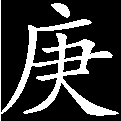
\includegraphics[width=3mm]{../Images/00004}此回栊翠品茶,怡红遇劫。盖妙玉虽以清净无为自守,而怪洁之癖未免有过,老妪只污得一杯,见而勿用,岂似玉兄日享洪福,竟至无以复加而不自知。故老妪眠其床,卧其席,酒屁熏其屋,却被袭人遮过,则仍用其床其席其屋。亦作者特为转眼不知身后事写来作戒,纨裤公子可不慎哉?}

{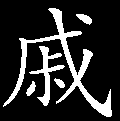
\includegraphics[width=3mm]{../Images/00005} \kaishu 任呼牛马从来乐,随分清高方可安。自古世情难意拟,淡妆浓抹有千般。立松轩。}

话说刘姥姥两只手比着说道:``花儿落了结个大倭瓜。''众人听了哄堂大笑起来。于是吃过门杯,因又逗趣笑道:``实告诉说罢,我的手脚子粗笨,又喝了酒,仔细失手打了这磁杯。有木头的杯取个子来,我便失了手,掉了地下也无碍。''众人听了,又笑起来。

凤姐儿听如此说,便忙笑道:``果真要木头的,我就取了来。可有一句话先说下:这木头的可比不得磁的,他都是一套,定要吃遍一套方使得。''刘姥姥听了心下敁敠道:``我方才不过是趣话取笑儿,谁知他果真竟有!我时常在村庄乡绅大家也赴过席,金杯银杯倒都也见过,从来没见有木头杯之说。哦,是了,想必是小孩子们使的木碗儿,不过诓我多喝两碗。别管他,横竖这酒蜜水儿似的,多喝点子也无妨。''{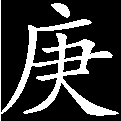
\includegraphics[width=3mm]{../Images/00004}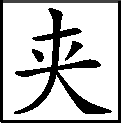
\includegraphics[width=3mm]{../Images/00012}\footnotesize \kaishu 为登厕伏脉。}想毕,便说:``取来再商量。''凤姐乃命丰儿:``到前面里间屋,书架子上有十个竹根套杯取来。''丰儿听了,答应才然要去,鸳鸯笑道:``我知道你这十个杯还小。况且你才说是木头的,这会子又拿了竹根子的来,倒不好看。不如把我们那里的黄杨根整抠的十个大套杯拿来,灌他十下子。''凤姐儿笑道:``更好了。''鸳鸯果命人取来。刘姥姥一看,又惊又喜:惊的是一连十个挨次大小分下来,那大的足似个小盆子,第十个极小的还有手里的杯子两个大;喜的是雕镂奇绝,一色山水、树木、人物,并有草字以及图印。因忙说道:``拿了那小的来就是了,怎么这样多?''凤姐儿笑道:``这个杯没有喝一个的理。我们家因没有这大量的,所以没人敢使他。姥姥既要,好容易寻了出来,必定要挨次吃一遍才使得。''刘姥姥唬的忙道:``这个不敢。好姑奶奶,饶了我罢。''{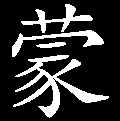
\includegraphics[width=3mm]{../Images/00006}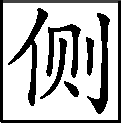
\includegraphics[width=3mm]{../Images/00011}\footnotesize \kaishu 挟炎的苦恼。}贾母、薛姨妈、王夫人知道他上了年纪的人,禁不起,忙笑道:``说是说,笑是笑,不可多吃了,只吃这头一杯罢。''刘姥姥道:``阿弥陀佛!我还是小杯吃罢。把这大杯收着,我带了家去慢慢的吃罢。''说的众人又笑起来。鸳鸯无法,只得命人满斟了一大杯,刘姥姥两手捧着喝。贾母薛姨妈都道:``慢些,不要呛了。''

薛姨妈又命凤姐儿布了菜。凤姐笑道:``姥姥要吃什么,说出名儿来,我搛了喂你。''刘姥姥道:``我知什么名儿,样样都是好的。''贾母笑道:``你把茄鲞搛些喂他。''凤姐儿听说,依言搛些茄鲞送入刘姥姥口中,因笑道:``你们天天吃茄子,也尝尝我们的茄子弄的可口不可口。''刘姥姥笑道:``别哄我了,茄子跑出这个味儿来了,我们也不用种粮食,只种茄子了。''众人笑道:``真是茄子,我们再不哄你。''刘姥姥诧异道:``真是茄子?我白吃了半日。姑奶奶再喂我些,这一口细嚼嚼。''凤姐果又搛了些放入口内。刘姥姥细嚼了半日,笑道:``虽有一点茄子香,只是还不像是茄子。告诉我是个什么法子弄的,我也弄着吃去。''凤姐儿笑道:``这也不难。你把才下来的茄子把皮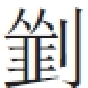
\includegraphics[width=4mm]{../images/00027}了,只要净肉,切成碎钉子,用鸡油炸了,再用鸡脯子肉并香菌、新笋、蘑菇、五香腐干、各色干果子,都切成钉子,拿鸡汤煨干,将香油一收,外加糟油一拌,盛在磁罐子里封严,要吃时拿出来,用炒的鸡瓜一拌就是。''刘姥姥听了,摇头吐舌说道:``我的佛祖!倒得十来只鸡来配他,怪道这个味儿!''

一面说笑,一面慢慢的吃完了酒,还只管细玩那杯。凤姐笑道:``还是不足兴,再吃一杯罢!''刘姥姥忙道:``了不得,那就醉死了。我因为爱这样范,亏他怎么作了。''鸳鸯笑道:``酒吃完了,到底这杯子是什么木的?''刘姥姥笑道:``怨不得姑娘不认得,你们在这金门绣户的,如何认得木头!我们成日家和树林子作街坊,困了枕着他睡,乏了靠着他坐,荒年间饿了还吃他,眼睛里天天见他,耳朵里天天听他,口儿里天天讲他,所以好歹真假,我是认得的。让我认一认。''{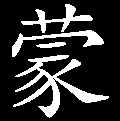
\includegraphics[width=3mm]{../Images/00006}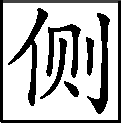
\includegraphics[width=3mm]{../Images/00011}\footnotesize \kaishu 好充懂得的来看。}一面说,一面细细端详了半日,道:``你们这样人家断没有那贱东西,那容易得的木头,你们也不收着了。我掂着这杯体重,断乎不是杨木,这一定是黄松做的。''众人听了,哄堂大笑起来。

只见一个婆子走来请问贾母,说:``姑娘们都到了藕香榭,请示下,就演罢还是再等一会子?''贾母忙笑道:``可是倒忘了他们,就叫他们演罢。''那个婆子答应去了。不一时,只听得箫管悠扬,笙笛并发。正值风清气爽之时,那乐声穿林度水而来,自然使人神怡心旷。

宝玉先禁不住,拿起壶来斟了一杯,一口饮尽。{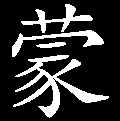
\includegraphics[width=3mm]{../Images/00006}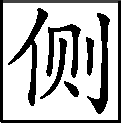
\includegraphics[width=3mm]{../Images/00011}\footnotesize \kaishu 作者似曾在座。}复又斟上,才要饮,只见王夫人也要饮,命人换暖酒,宝玉连忙将自己的杯捧了过来,送到王夫人口边,{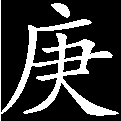
\includegraphics[width=3mm]{../Images/00004}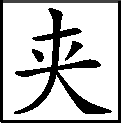
\includegraphics[width=3mm]{../Images/00012}\footnotesize \kaishu 妙极!忽写宝玉如此,便是天地间母子之至情至性。献芹之民之意,令人酸鼻。}王夫人便就他手内吃了两口。一时暖酒来了,宝玉仍归旧坐,王夫人提了暖壶下席来,众人皆都出了席,薛姨妈也立起来,贾母忙命李、凤二人接过壶来:``让你姑妈坐了,大家才便。''王夫人见如此说,方将壶递与凤姐,自己归坐。贾母笑道:``大家吃上两杯,今日着实有趣。''说着擎杯让薛姨妈,又向湘云宝钗道:``你姐妹两个也吃一杯。你妹妹虽不大会吃,也别饶他。''说着自己已干了。湘云、宝钗、黛玉也都干了。当下刘姥姥听见这般音乐,且又有了酒,越发喜的手舞足蹈起来。宝玉因下席过来向黛玉笑道:``你瞧刘姥姥的样子。''黛玉笑道:``当日圣乐一奏,百兽率舞,如今才一牛耳。''{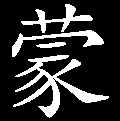
\includegraphics[width=3mm]{../Images/00006}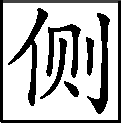
\includegraphics[width=3mm]{../Images/00011}\footnotesize \kaishu 随笔写来,趣极。}众姐妹都笑了。

须臾乐止,薛姨妈出席笑道:``大家的酒想也都有了,且出去散散再坐罢。''贾母也正要散散,于是大家出席,都随着贾母游玩。贾母因要带着刘姥姥散闷,遂携了刘姥姥至山前树下盘桓了半晌,又说与他这是什么树,这是什么石,这是什么花。刘姥姥一一的领会,又向贾母道:``谁知城里不但人尊贵,连雀儿也是尊贵的。偏这雀儿到了你们这里,他也变俊了,也会说话了。''众人不解,因问什么雀儿变俊了,会讲话。刘姥姥道:``那廊下金架子上站的绿毛红嘴是鹦哥儿,我是认得的。那笼子里的黑老鸹子怎么又长出凤头来,也会说话呢。''众人听了都笑将起来。

一时只见丫鬟们来请用点心。贾母道:``吃了两杯酒,倒也不饿。也罢,就拿了这里来,大家随便吃些罢。''丫鬟便去抬了两张几来,又端了两个小捧盒。揭开看时,每个盒内两样:这盒内一样是藕粉桂糖糕,一样是松穰鹅油卷;那盒内一样是一寸来大的小饺儿,贾母因问什么馅儿,婆子们忙回是螃蟹的。贾母听了,皱眉说:``这油腻腻的,谁吃这个!''那一样是奶油炸的各色小面果,也不喜欢。因让薛姨妈吃,薛姨妈只拣了一块糕;贾母拣了一个卷子,只尝了一尝,剩的半个递与丫鬟了。

刘姥姥因见那小面果子都玲珑剔透,便拣了一朵牡丹花样的笑道:``我们那里最巧的姐儿们,也不能铰出这么个纸的来。我又爱吃,又舍不得吃,包些家去给他们做花样子去倒好。''{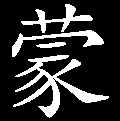
\includegraphics[width=3mm]{../Images/00006}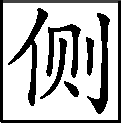
\includegraphics[width=3mm]{../Images/00011}\footnotesize \kaishu 世上竟有这样人。}众人都笑了。贾母道:``家去我送你一坛子。你先趁热吃这个罢。''别人不过拣各人爱吃的一两点就罢了;刘姥姥原不曾吃过这些东西,且都作的小巧,不显盘堆的,他和板儿每样吃了些,就去了半盘子。剩的,凤姐又命攒了两盘并一个攒盒,与文官等吃去。

忽见奶子抱了大姐儿来,大家哄他顽了一会。那大姐儿因抱着一个大柚子玩的,忽见板儿抱着一个佛手,便也要佛手。{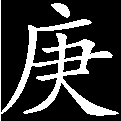
\includegraphics[width=3mm]{../Images/00004}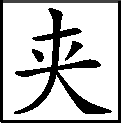
\includegraphics[width=3mm]{../Images/00012}\footnotesize \kaishu 小儿常情,遂成千里伏线。}丫鬟哄他取去,大姐儿等不得,便哭了。众人忙把柚子与了板儿,{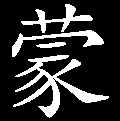
\includegraphics[width=3mm]{../Images/00006}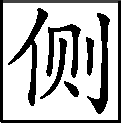
\includegraphics[width=3mm]{../Images/00011}\footnotesize \kaishu 伏线千里。}将板儿的佛手哄过来与他才罢。那板儿因顽了半日佛手,此刻又两手抓着些果子吃,又忽见这柚子又香又圆,更觉好顽,且当球踢着玩去,也就不要佛手了。{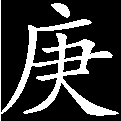
\includegraphics[width=3mm]{../Images/00004}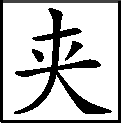
\includegraphics[width=3mm]{../Images/00012}\footnotesize \kaishu 柚子即今香{(团)}{[}橼{]}之属也,应与``缘''通。佛手者,正指迷津者也。以小儿之戏暗透前后通部脉络,隐隐约约,毫无一丝漏泄,岂独为刘姥姥之俚言博笑而有此一大回文字哉? 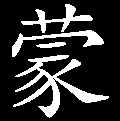
\includegraphics[width=3mm]{../Images/00006}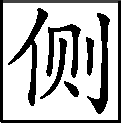
\includegraphics[width=3mm]{../Images/00011}\footnotesize \kaishu 画工。}

当下贾母等吃过茶,又带了刘姥姥至栊翠庵来。妙玉忙接了进去。至院中见花木繁盛,贾母笑道:``到底是他们修行的人,没事常常修理,比别处越发好看。''一面说,一面便往东禅堂来。妙玉笑往里让,贾母道:``我们才都吃了酒肉,你这里头有菩萨,冲了罪过。我们这里坐坐,把你的好茶拿来,我们吃一杯就去了。''妙玉听了,忙去烹了茶来。宝玉留神看他是怎么行事。只见妙玉亲自捧了一个海棠花式雕漆填金云龙献寿的小茶盘,里面放一个成窑五彩小盖钟,捧与贾母。贾母道:``我不吃六安茶。''妙玉笑说:``知道。这是老君眉。''贾母接了,又问是什么水。妙玉笑回:``是旧年蠲的雨水。''贾母便吃了半盏,便笑着递与刘姥姥说:``你尝尝这个茶。''刘姥姥便一口吃尽,笑道:``好是好,就是淡些,再熬浓些更好了。''贾母众人都笑起来。然后众人都是一色官窑脱胎填白盖碗。

那妙玉便把宝钗和黛玉的衣襟一拉,二人随他出去,宝玉悄悄的随后跟了来。只见妙玉让他二人在耳房内,宝钗坐在榻上,黛玉便坐在妙玉的蒲团上。妙玉自向风炉上扇滚了水,另泡一壶茶。宝玉便走了进来,笑道:``偏你们吃梯己茶呢。''二人都笑道:``你又赶了来飺茶吃。这里并没你的。''妙玉刚要去取杯,只见道婆收了上面的茶盏来。妙玉忙命:``将那成窑的茶杯别收了,搁在外头去罢。''宝玉会意,知为刘姥姥吃了,他嫌脏不要了。又见妙玉另拿出两只杯来。一个旁边有一耳,杯上镌着``??瓟斝''三个隶字,后有一行小真字是``晋王恺珍玩'',又有``宋元丰五年四月眉山苏轼见于秘府''一行小字。妙玉便斟了一斝,递与宝钗。那一只形似钵而小,也有三个垂珠篆字,镌着``点犀??''。妙玉斟了一??与黛玉。仍将前番自己常日吃茶的那只绿玉斗来斟与宝玉。

宝玉笑道:``常言`世法平等',他两个就用那样古玩奇珍,我就是个俗器了。''妙玉道:``这是俗器?不是我说狂话,只怕你家里未必找的出这么一个俗器来呢。''宝玉笑道:``俗说`随乡入乡',到了你这里,自然把那金玉珠宝一概贬为俗器了。''妙玉听如此说,十分欢喜,遂又寻出一只九曲十环一百二十节蟠虬整雕竹根的一个大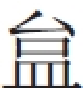
\includegraphics[width=4mm]{../images/00013}出来,笑道:``就剩了这一个,你可吃的了这一海?''宝玉喜的忙道:``吃的了。''妙玉笑道:``你虽吃的了,也没这些茶糟蹋。{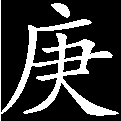
\includegraphics[width=3mm]{../Images/00004}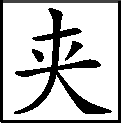
\includegraphics[width=3mm]{../Images/00012}\footnotesize \kaishu 茶下``糟蹋''二字,成窑杯已不屑再要,妙玉真清洁高雅,然亦怪谲孤僻甚矣。实有此等人物,但罕耳。}岂不闻`一杯为品,二杯即是解渴的蠢物,三杯便是饮牛饮骡了'。你吃这一海便成什么?''说的宝钗、黛玉、宝玉都笑了。妙玉执壶,只向海内斟了约有一杯。宝玉细细吃了,果觉轻浮无比,赏赞不绝。妙玉正色道:``你这遭吃的茶是托他两个福,独你来了,我是不给你吃的。''宝玉笑道:``我深知道的,我也不领你的情,只谢他二人便是了。''妙玉听了,方说:``这话明白。''

黛玉因问:``这也是旧年的雨水?''妙玉冷笑道:``你这么个人,竟是大俗人,连水也尝不出来。这是五年前我在玄墓蟠香寺住着,收的梅花上的雪,共得了那一鬼脸青的花瓮一瓮,总舍不得吃,埋在地下,{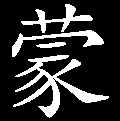
\includegraphics[width=3mm]{../Images/00006}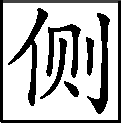
\includegraphics[width=3mm]{../Images/00011}\footnotesize \kaishu 妙手。层层叠起,竟能以他人所画之天王作众神矣。}今年夏天才开了。我只吃过一回,这是第二回了。你怎么尝不出来?隔年蠲的雨水那有这样轻浮,如何吃得。''黛玉知他天性怪僻,不好多话,亦不好多坐,吃过茶,便约着宝钗走了出来。

宝玉和妙玉陪笑道:``那茶杯虽然脏了,白撂了岂不可惜?依我说,不如就给那贫婆子罢,他卖了也可以度日。你道可使得。''妙玉听了,想了一想,点头说道:``这也罢了。幸而那杯子是我没吃过的,若我使过,我就砸碎了也不能给他。{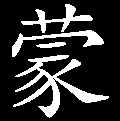
\includegraphics[width=3mm]{../Images/00006}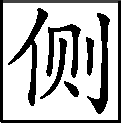
\includegraphics[width=3mm]{../Images/00011}\footnotesize \kaishu 更奇!世上我也见过此等人。}你要给他,我也不管你,只交给你,快拿了去罢。''宝玉道:``自然如此,你那里和他说话授受去,越发连你也脏了。{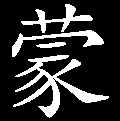
\includegraphics[width=3mm]{../Images/00006}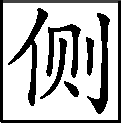
\includegraphics[width=3mm]{../Images/00011}\footnotesize \kaishu 人若忘形,最喜此等言语。}只交与我就是了。''妙玉便命人拿来递与宝玉。宝玉接了,又道:``等我们出去了,我叫几个小幺儿来河里打几桶水来洗地如何?''妙玉笑道:``这更好了,只是你嘱咐他们,抬了水只搁在山门外头墙根下,别进门来。''{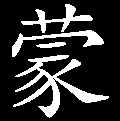
\includegraphics[width=3mm]{../Images/00006}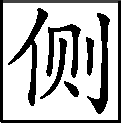
\includegraphics[width=3mm]{../Images/00011}\footnotesize \kaishu 偏于无可写处,深入一层。}宝玉道:``这是自然的。''说着,便袖着那杯,递与贾母房中小丫头拿着,说:``明日刘姥姥家去,给他带去罢。''交代明白,贾母已经出来要回去。妙玉亦不甚留,送出山门,回身便将门闭了。不在话下。

且说贾母因觉身上乏倦,便命王夫人和迎春姊妹陪了薛姨妈去吃酒,自己便往稻香村来歇息。凤姐忙命人将小竹椅抬来,贾母坐上,两个婆子抬起,凤姐李纨和众丫鬟婆子围随去了,不在话下。这里薛姨妈也就辞出。王夫人打发文官等出去,将攒盒散与众丫鬟们吃去,自己便也乘空歇着,随便歪在方才贾母坐的榻上,命一个小丫头放下帘子来,又命他捶着腿,吩咐他:``老太太那里有信,你就叫我。''说着也歪着睡着了。

宝玉湘云等看着丫鬟们将攒盒搁在山石上,也有坐在山石上的,也有坐在草地下的,也有靠着树的,也有傍着水的,倒也十分热闹。一时又见鸳鸯来了,要带着刘姥姥各处去逛,{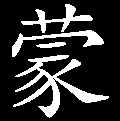
\includegraphics[width=3mm]{../Images/00006}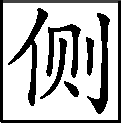
\includegraphics[width=3mm]{../Images/00011}\footnotesize \kaishu 又另是一番气象。}众人也都赶着取笑。一时来至``省亲别墅''的牌坊底下,刘姥姥道:``嗳呀!这里还有个大庙呢。''说着,便爬下磕头。众人笑弯了腰。刘姥姥道:``笑什么?这牌楼上字我都认得。我们那里这样的庙宇最多,都是这样的牌坊,那字就是庙的名字。''众人笑道:``你认得这是什么庙?''刘姥姥便抬头指那字道:``这不是`玉皇宝殿'四字?''众人笑的拍手打脚,还要拿他取笑。刘姥姥觉得腹内一阵乱响,忙的拉着一个小丫头,要了两张纸就解衣。众人又是笑,又忙喝他``这里使不得!''忙命一个婆子带了东北上去了。那婆子指与地方,便乐得走开去歇息。

那刘姥姥因喝了些酒,他脾气不与黄酒相宜,且吃了许多油腻饮食,发渴多喝了几碗茶,不免通泻起来,蹲了半日方完。及出厕来,酒被风禁,且年迈之人,蹲了半天,忽一起身,只觉得眼花头眩,辨不出路径。四顾一望,皆是树木山石楼台房舍,却不知那一处是往那里去的了,只得认着一条石子路慢慢的走来。及至到了房舍跟前,又找不着门,再找了半日,忽见一带竹篱,刘姥姥心中自忖道:``这里也有扁豆架子。''

一面想,一面顺着花障走了来,得了一个月洞门进去。只见迎面忽有一带水池,只有七八尺宽,石头砌岸,里边碧浏清水流往那边去了,{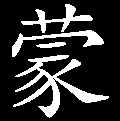
\includegraphics[width=3mm]{../Images/00006}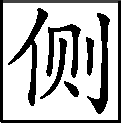
\includegraphics[width=3mm]{../Images/00011}\footnotesize \kaishu 借刘姥姥醉中,写境中景。}上面有一块白石横架在上面。刘姥姥便度石过去,顺着石子甬路走去,转了两个弯子,只见有一房门。于是进了房门,只见迎面一个女孩儿,满面含笑迎了出来。刘姥姥忙笑道:``姑娘们把我丢下来了,要我碰头碰到这里来。''说了,只觉那女孩儿不答。刘姥姥便赶来拉他的手,``咕咚''一声,便撞到板壁上,把头碰的生疼。细瞧了一瞧,原来是一幅画儿。刘姥姥自忖道:``原来画儿有这样活凸出来的。''一面想,一面看,一面又用手摸去,却是一色平的,点头叹了两声。一转身方得了一个小门,门上挂着葱绿撒花软帘。

刘姥姥掀帘进去,抬头一看,只见四面墙壁玲珑剔透,琴剑瓶炉皆贴在墙上,锦笼纱罩,金彩珠光,连地下踩的砖,皆是碧绿凿花,竟越发把眼花了,找门出去,那里有门?左一架书,右一架屏。刚从屏后得了一门转去,只见他亲家母也从外面迎了进来。刘姥姥诧异,忙问道:``你想是见我这几日没家去,亏你找我来。那一位姑娘带你进来的?''他亲家只是笑,不还言。刘姥姥笑道:``你好没见世面,见这园里的花好,你就没死活戴了一头。''他亲家也不答。便心下忽然想起:``常听大富贵人家有一种穿衣镜,这别是我在镜子里头呢罢。''说毕伸手一摸,再细一看,可不是,四面雕空紫檀板壁将镜子嵌在中间。因说:``这已经拦住,如何走出去呢?''一面说,一面只管用手摸。

这镜子原是西洋机括,可以开合。不意刘姥姥乱摸之间,其力巧合,便撞开消息,掩过镜子,露出门来。刘姥姥又惊又喜,迈步出来,忽见有一副最精致的床帐。他此时又带了七八分醉,又走乏了,便一屁股坐在床上,只说歇歇,不承望身不由己,前仰后合的,朦胧着两眼,一歪身就睡熟在床上。

且说众人等他不见,板儿见没了他姥姥,急的哭了。众人都笑道:``别是掉在茅厕里了?快叫人去瞧瞧。''因命两个婆子去找,回来说没有。众人各处搜寻不见。袭人敁敠其道路:``是他醉了迷了路,顺着这一条路往我们后院子里去了。若进了花障子到后房门进去,虽然碰头,还有小丫头们知道;若不进花障子再往西南上去,若绕出去还好,若绕不出去,可够他绕回子好的。我且瞧瞧去。''一面想,一面回来,进了怡红院便叫人,谁知那几个房子里小丫头已偷空顽去了。

袭人一直进了房门,转过集锦槅子,就听的鼾齁如雷。忙进来,只闻见酒屁臭气,满屋一瞧,只见刘姥姥扎手舞脚的仰卧在床上。袭人这一惊不小,慌忙赶上来将他没死活的推醒。那刘姥姥惊醒,睁眼见了袭人,连忙爬起来道:``姑娘,我失错了!并没弄脏了床帐。''一面说,一面用手去掸。

袭人恐惊动了人,被宝玉知道了,只向他摇手,不叫他说话。忙将鼎内贮了三四把百合香,仍用罩子罩上。些须收拾收拾,所喜不曾呕吐,忙悄悄的笑道:``不相干,有我呢。你随我出来。''{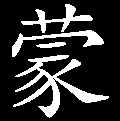
\includegraphics[width=3mm]{../Images/00006}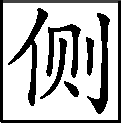
\includegraphics[width=3mm]{../Images/00011}\footnotesize \kaishu 这方是袭人的平素,笔至此不得不屈,再增支派则累{[}赘{]}矣。}刘姥姥跟了袭人,出至小丫头们房中,命他坐了,向他说道:``你就说醉倒在山子石上打了个盹儿。''刘姥姥答应知道。{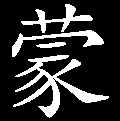
\includegraphics[width=3mm]{../Images/00006}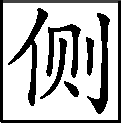
\includegraphics[width=3mm]{../Images/00011}\footnotesize \kaishu 总是恰好便住。}又与他两碗茶吃,方觉酒醒了,因问道:``这是那个小姐的绣房,这样精致?我就像到了天宫里的一样。''袭人微微笑道:``这个么,是宝二爷的卧室。''那刘姥姥吓的不敢作声。袭人带他从前面出去,见了众人,只说他在草地下睡着了,带了他来的。众人都不理会,也就罢了。

一时贾母醒了,就在稻香村摆晚饭。贾母因觉懒懒的,也不吃饭,便坐了竹椅小敞轿,回至房中歇息,命凤姐儿等去吃饭。他姊妹方复进园来。要知端的------

{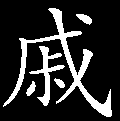
\includegraphics[width=3mm]{../Images/00005} \kaishu 总评:刘姥姥之憨从利,妙玉尼之怪图名,宝玉之奇、黛玉之妖亦自敛迹。是何等画工,能将他人之天王,作我卫护之神祗?文技至此,可为至矣!}
